\documentclass{article}

\usepackage{graphicx} % Required for inserting images
\usepackage{amsmath} % useful
\usepackage{amsfonts} % fonts like \mathbb{R} among others
\usepackage{amssymb}
\usepackage{amsthm} % used for writing lemmas/theorems/etc
\usepackage{tikz} % for visual tools
\usepackage{authblk}
\usepackage{enumitem}
\usepackage{url}
\usepackage{array}
\usepackage{subfig}
\usepackage{float} % i hate images
\numberwithin{equation}{section}
\usepackage[margin=1in]{geometry}

\newtheorem{theorem}{Theorem}[section]
\newtheorem{corollary}{Corollary}[theorem]
\newtheorem{lemma}[theorem]{Lemma}
\newtheorem{proposition}[theorem]{Proposition}

\theoremstyle{definition}
\newtheorem{definition}{Definition}[section]
\newtheorem{remark}{Remark}[theorem]

\title{MATH60025 Computational PDEs Coursework 2}
\author{
CID: 02033585
}
\date{}

\newcommand{\R}{\mathbb{R}}
\newcommand{\C}{\mathbb{C}}
\newcommand{\Q}{\mathbb{Q}}
\newcommand{\pr}{\mathbb{P}}
\newcommand{\E}{\mathbb{E}}
\newcommand{\dm}{\mathrm{d}}

\newcommand{\mc}[1]{\mathcal{#1}}
\newcommand{\pspace}{(\Omega, \mathcal{F}, \mathbb{P})}

\newcommand{\sm}{\setminus}

\newcommand{\ie}{\textit{i}.\textit{e}. }
\newcommand{\eg}{\textit{e}.\textit{g}. }

\newcommand{\dd}[2]{\frac{\mathrm{d} #1}{\mathrm{d} #2}}
\newcommand{\ddn}[3]{\frac{\mathrm{d}^{#3} #1}{\mathrm{d}^{#3} #2}}
\newcommand{\pp}[2]{\frac{\partial #1}{\partial #2}}
\newcommand{\ppn}[3]{\frac{\partial^{#1} #2}{\partial #3^{#1}}}


\newcommand{\eps}{\varepsilon}
\begin{document}

\maketitle

\section{Part A}


\begin{figure}[H]
    \centering
    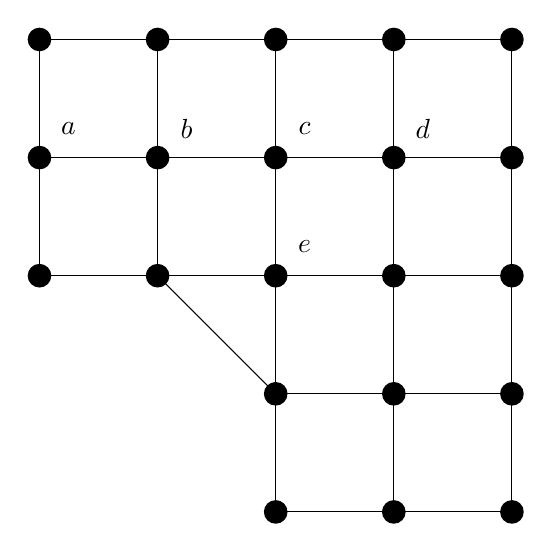
\begin{tikzpicture}[scale=1.5]
        % Nodes
        \foreach \x in {0,1,...,4} {
            \foreach \y in {0,1,...,4} {
                \ifnum\x>1
                    \fill (\x,\y) circle (0.1);
                \else
                    \ifnum\y>1
                        \fill (\x,\y) circle (0.1);
                    \fi
                \fi
            }
        }
        
        % Edges
        \foreach \x in {0,1,...,3} {
            \foreach \y in {2,3,4} {
                \draw (\x,\y) -- (\x+1,\y);
            }
        }
        \foreach \x in {2,3,4} {
            \foreach \y in {0,1,...,3} {
                \draw (\x,\y) -- (\x,\y+1);
            }
        }

        \foreach \x in {0,1} {
            \foreach \y in {2,3} {
                \draw (\x,\y) -- (\x,\y+1);
            }
        }
        \foreach \x in {2,3} {
            \foreach \y in {0,1} {
                \draw (\x,\y) -- (\x+1,\y);
            }
        }

        \draw (1,2) -- (2,1);

        \node at (3+0.245,3+0.245) {$d$};
        \node at (2+0.245,2+0.245) {$e$};
        \node at (2+0.245,3+0.245) {$c$};
        \node at (1+0.245,3+0.245) {$b$};
        \node at (0+0.245,3+0.245) {$a$};
    \end{tikzpicture}
    \caption{Coarse grid, with five unknown values.}
    \label{fig:grid}
\end{figure}


Everywhere except for $a$, we use the second-order central differences $\delta^2_x$ and $\delta^2_y$ to approximate $u_{xx} + u_{yy}$.
\begin{align}
    \frac{1}{h^2} \left(
        4U_{i,j} - U_{i+1,j} - U_{i-1,j} - U_{i,j+1} - U_{i,j-1}
    \right)
    = 4
\end{align}
At point $a$ we enforce the boundary condition with the $O(h^2)$ accurate central difference (with $i$ pointing in the positive $x$ direction)
\begin{equation}
    \pp{u_{i,j}}{x}=\frac{u_{i+1,j}-u_{i-1,j}}{2h}
\end{equation}
This introduces a ficticious point to the left of $a$, which must have value equal to $b$ by the above. Combined with the finite difference approximation for $u_{xx} + u_{yy} + 4$, we get the equation

\begin{equation}
    4a - b - b - 0 - 1 = 4h^2
\end{equation}


We therefore get the system of equations for the five variables, where we used the symmetry of the grid (for example, the point to the right of $e$ has the same value as $c$):
\begin{align}
    4a - b - b - 0 - 1 &= 4h^2 \\
    4b - a - c - 1 &= 4h^2 \\
    4c - b - d - e &= 4h^2 \\
    4d - 2c &= 4h^2 \\
    4e - 2c -2 &= 4h^2
\end{align}
Equivalently in matrix form:
\begin{equation}
    \begin{pmatrix}
        4 & -2 & 0 & 0 & 0\\ 
        -1 & 4 & -1 & 0 & 0\\ 
        0 & -1 & 4 & -1 & -1\\ 
        0 & 0 & -2 & 4 & 0\\ 
        0 & 0 & -2 & 0 & 4
        \end{pmatrix}U=\begin{pmatrix}
        4h^2 + 1\\ 
        4h^2 + 1\\ 
        4h^2\\ 
        4h^2\\
        4h^2 + 2
        \end{pmatrix}
\end{equation}
\subsection{Direct Method}
Solving this system with $h=\frac12$ yields the solution with direct method \path{direct_method_A} as

\begin{table}[H]
    \centering
    \begin{tabular}{|m{2.159cm}|m{2.159cm}|m{2.159cm}|m{2.159cm}|m{2.159cm}|}
    \hline
    $a$ & $b$ & $c$ & $d$  & $e$  \\ \hline
    1.0 & 1.0 & 1.0 & 0.75 & 1.25 \\ \hline
    \end{tabular}
\end{table}

\subsection{Jacobi Method}
We iterate starting with $a_0,b_0,c_0,d_0,e_0 = 0$ and equations
\begin{align}
    4a_1 &= 2 + b_0\\
    4b_1 &= 2 +a_0+c_0\\
    4c_1 &= 1 +b_0+d_0+e_0\\
    4d_1 &= 1+ 2c_0 \\
    4e_1 &= 3+2c_0
\end{align}
Once all values are calculated, we replace $a_0$ with $a_1$, $b_0$ with $b_1$ etc. simultaneously, each iteration.
If we let $D$ be the diagonal part of $A$ and $C$ be the off-diagonal entries, we can rewrite this as the matrix system
\begin{equation}
    U^{j+1} = D^{-1}(b - CU^j)
\end{equation}
The function is located at \path{jacobi_method_A}.


\subsection{Gauss-Seidel Method}
We again iterate starting with $a,b,c,d,e = 0$ and equations, where we use new values as soon as possible.
\begin{align}
    4a &= 2 + b\\
    4b &= 2 +a+c\\
    4c &= 1 +b+d+e\\
    4d &= 1+ 2c \\
    4e &= 3+2c
\end{align}
We define further matrices $L$ and $V$ as the lower and upper triangular parts of $C$. Using these matrices, the scheme can be written in matrix form as
\begin{equation}
    U^{j+1} = (D+L)^{-1}(b - VU^j)
\end{equation}
The function is written at \path{gauss_seidel_method_A}.

\subsection{Successive over-relaxation method}
The successive over-relaxation scheme is given by iterates

\begin{equation}
    U^{j+1} = U^{j} + w (D + L)^{-1} r^j
\end{equation}

where $w$ is a parameter to be chosen (the case of Gauss-Seidel is given by $w=1$) and $r^j$ is the residual $b - AU^j$.
The function is written at \path{SOR_method_A}.

\subsection{Convergence of the three methods}
\begin{figure}[H]
    \centering
    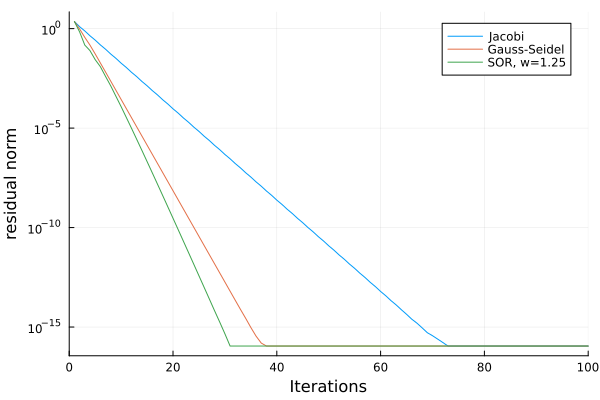
\includegraphics[width=0.496\textwidth]{fig1.png}
    \caption{Plot of residual norm over iterations, for the three different iterative methods.}
    \label{fig:afig_1}
\end{figure}
In Figure \ref{fig:afig_1} we see that Jacobi reduces the residual norm by a factor of $10^{-15}$ in about $65$ iterations, Gauss-Seidel in $40$ and SOR, $w=1.25$ in about $25$. The following section will show how these values are a consequence of the different spectral radii of the iteration matrices.

For Jacobi, the iteration matrix is $D^{-1}(L+V)$, which has spectral radius $\rho_J \approx 0.5896$ (calculated using \path{spectral_radius}) in this case. Similarly, $\rho_{GS}$ is calculated with $(D+L)^{-1}V$ and is approximately $0.3476$.

To derive the iteration matrix for SOR, we start with the scheme and rearrange into a form such that $A = B+C$ with $BU^j = b - CU^j$.

\begin{align}
    U^{j+1} &= U^j + w(D+L)^{-1}r^j \\
    U^{j+1} &= U^j + w(D+L)^{-1}b - w(D+L)^{-1}VU^j-w U^j\\
    \frac 1w (D+L)U^{j+1} &= b - \left(\frac{w-1}{w}(D+L) + V\right)U^j
\end{align}
The iteration matrix can be read off as
\begin{equation}
    \label{eq:sor_it_mat}
    (w-1)I + w(D+L)^{-1}V
\end{equation}

For $w=1.25$, the spectral radius is $\approx 0.25$.


With these spectral radii, we can estimate the number of iterations needed to reduce the residual by a factor of $10^{-15}$, since the magnitude of the error exponentially decreases. The formula is then
\begin{equation}
    \text{iterations} \approx -\frac{15}{\log_{10}(\rho)}
\end{equation}
Plugging in the three spectral radii, we get approximately 65 iterations for Jacobi, 33 iterations for Gauss-Seidel and 25 iterations for SOR, $w=1.25$, which is very close to what we observe in Figure \ref{fig:afig_1}.

\subsection{Optimal parameter for SOR}
We can use the previous formula in Equation \eqref{eq:sor_it_mat} to find the optimal parameter by minimising
\begin{equation}
    \rho((w-1)I + w(D+L)^{-1}V)
\end{equation}

\begin{figure}[H]
    \centering
    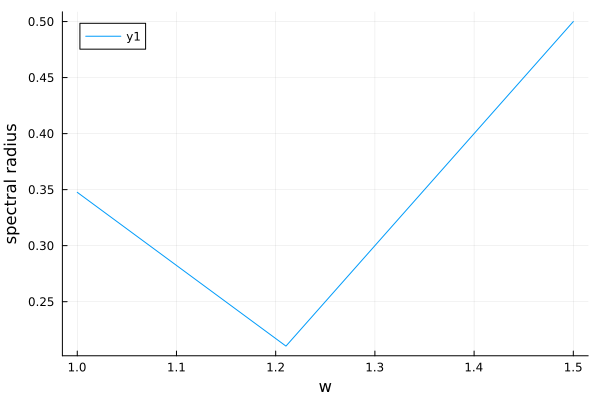
\includegraphics[width=0.496\textwidth]{fig2.png}
    \caption{Plot of spectral radius of iteration matrix of SOR, with $w$ varying.}
    \label{fig:afig_2}
\end{figure}
Figure \ref{fig:afig_2} shows the spectral radius as $w$ varies. There is a clear minimum at around $1.2103$, and we find that the spectral radius at this point is $\approx 0.2104$. We plot below the convergence rate at this point, compared to neighbouring values of $w$. As expected $w$ minimises the iteration count within a margin of error (Here, iteration count was measured by checking if the residual was below a tolerance $10^{-14}$).

\begin{figure}[H]
    \centering
    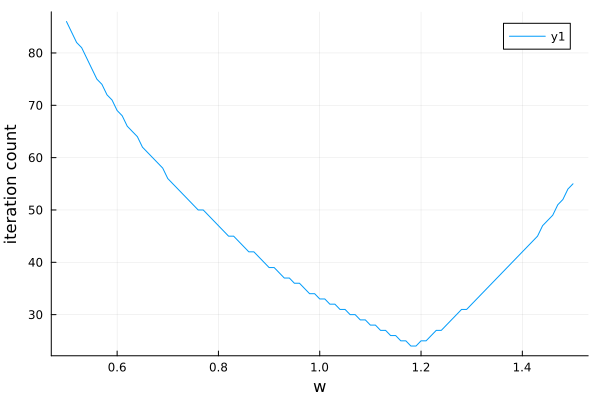
\includegraphics[width=0.496\textwidth]{fig2h.png}
    \caption{Plot of iteration count of SOR, with $w$ varying.}
    \label{fig:fig2h}
\end{figure}

\section{Part B}

\begin{figure}[H]
    \centering
    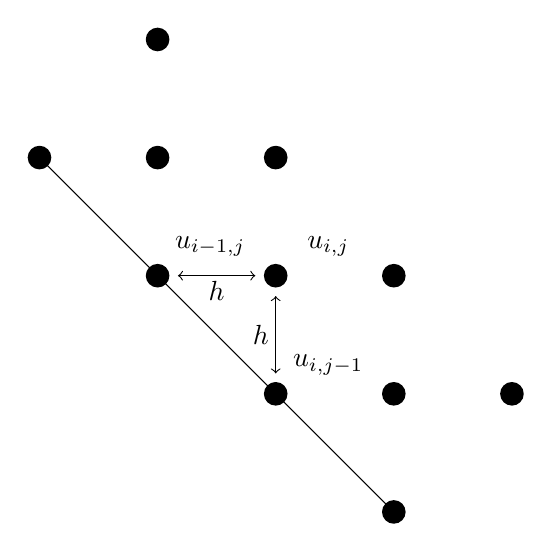
\begin{tikzpicture}[scale=1.5]
        \fill (3,0) circle (0.1);
        \fill (3,1) circle (0.1);
        \fill (4,1) circle (0.1);

        \fill (2,1) circle (0.1);
        \fill (2,2) circle (0.1);
        \fill (3,2) circle (0.1);

        \fill (1,2) circle (0.1);
        \fill (1,3) circle (0.1);
        \fill (2,3) circle (0.1);

        \fill (0,3) circle (0.1);
        \fill (1,4) circle (0.1);
        
        

        \draw (1,2) -- (2,1);
        \draw (3,0) -- (2,1);
        \draw (1,2) -- (0,3);
        \draw[<->] (1+0.1723,2) -- (2-0.1723,2);
        \draw[<->] (2,2-0.1723) -- (2,1+0.1723);

        \node at (1.5,2-0.1256) {$h$};
        \node at (2-0.1256,1.5) {$h$};

        \node at (2+0.445,1+0.245) {$u_{i,j-1}$};
        \node at (1+0.445,2+0.245) {$u_{i-1,j}$};
        \node at (2+0.445,2+0.245) {$u_{i,j}$};

    \end{tikzpicture}
    \caption{$q-v$ boundary discretisation in the case $\Delta x = \Delta y$. The values $u_{i-1,j}$ and $u_{i,j-1}$ are known exactly, as they lie directly on the boundary.}
    \label{fig:grid2}
\end{figure}
Throughout this part, we assume that $\Delta x$ and $\Delta y$ both divide into $0.5$ an integer number of times, for simplicity. In addition, we also assume they are equal, to make use of the symmetry condition. The discretisation near the boundary therefore looks like Figure \ref{fig:grid2}. In this case, for any point $u_{i,j}$ close to the boundary, $u_{i,j-1}$ and $u_{i-1,j}$ lie \textbf{exactly} on the boundary, and thus have known values. As such, we can apply the usual finite difference formula without worrying about irregular boundaries and adaptive stencils.

\subsection{Gauss-Seidel (Single Grid)}
Function written at \path{gauss_seidel_method_B} (as a special case of SOR), with parameter $N$ detailing how many points in both $x$ and $y$ directions.

We solve for only the values on half of the domain, reflecting the values along the line of symmetry. Convergence is monitored using the pseudo-residual $\|u_{new} - u_{old}\|$, and we determine convergence when this residual is lower than $10^{-12}$. A solution calculated using this method is contoured at Figure \ref{fig:fig3}.

\subsection{Successive Over-relaxation}
Function written at \path{SOR_method_B}, with the same grid and convergence criterion as described before. We will determine the optimal $w$ parameter in two ways.

\subsubsection{Testing with a loose tolerance.}
First, we estimate by testing different values $w$ and recording the number of iterations it takes for the residual to drop below $10^{-3}$ (function at \path{optimal_SOR_parameter_test}). An example plot is given for different $N$ values (Figure \ref{fig:figsor1}).

\begin{figure}[H]
    \centering
    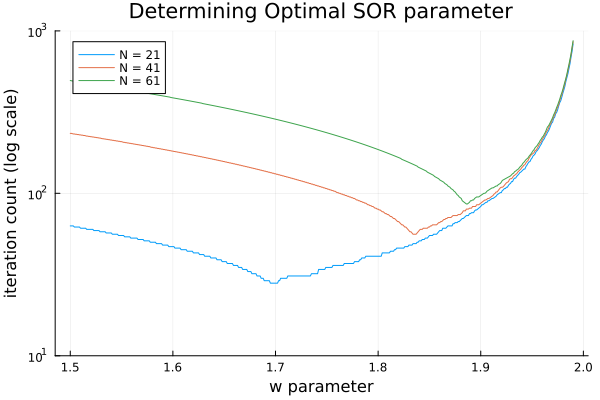
\includegraphics[width=0.49\textwidth]{figsor1.png}
    \caption{Iteration count as the SOR parameter $w$ is varied, for different $N$.}
    \label{fig:figsor1}
\end{figure}

The table below shows the optimal parameters obtained via this method (testing every value of $w$ in the interval $[1.5, 1.99]$ with $0.001$ spacing).

\begin{table}[H]
    \centering
    \begin{tabular}{|l|l|l|l|l|l|}
    \hline
    $N$       & 21    & 41    & 61    & 81    & 101   \\ \hline
    $w_{opt}$ & 1.695 & 1.834 & 1.886 & 1.913 & 1.929 \\ \hline
    \end{tabular}
\end{table}


\subsubsection{Asymptotic spectral radius}
Secondly, we estimate the optimal parameter by using the asymptotic formula for the spectral radius of the Gauss-Seidel iteration matrix, that is:

\begin{align}
    \rho_{GS} &\approx 1 - \frac{\pi^2}{N^2} \\
    w_{opt} &\approx \frac{2}{1 + \sqrt{1-\rho_{GS}^2}}
\end{align}
The above formulas were taken from the lecture notes (Function calculating this is written at \path{optimal_SOR_parameter_asym}). The second formula is only exact for real symmetric block tridiagonal matrices, which typically occur when the domain the PDE is being solved on is square. However, we will see later on that nevertheless, the formula is a good guess for the optimal parameter with a fraction of the computational cost.

\subsubsection{Combination and comparison between methods}
The first method comes with the disadvantage that it becomes expensive to compute for large $N$, and so it is desirable to reduce the size of the interval search space to speed up computation time. On the other hand, the asymptotic formula is easy to compute, but is only a heuristic.

This suggests a combination of the above two methods: use asymptotics to get a small interval in which to search for the optimal parameter.

Using this method, we can see how accurate the asymptotic formula is by plotting $w_{opt}$ for larger $N$ (Figure \ref{fig:figsor2}). We see that the asymptotic formula obtains a decent guess with barely any computational cost. Another thing we observe is that the optimal parameter seems to be approaching $2$ with higher and higher $N$. This is a consequence of the spectral radius of the iteration matrix approaching $1$ as $N \to \infty$ (the same reason the iterative method converges slower for large $N$).

\begin{figure}[H]
    \centering
    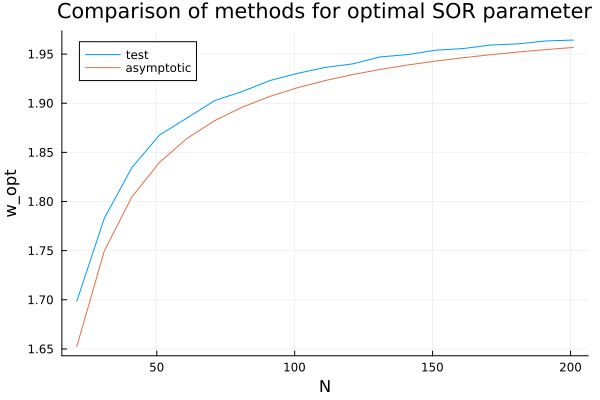
\includegraphics[width=0.49\textwidth]{figsor2.png}
    \caption{Comparison between the asymptotic value of $w_{opt}$ with the value obtained from testing the convergence rate.}
    \label{fig:figsor2}
\end{figure}

A solution calculated using this method is contoured at Figure \ref{fig:fig4}.









\subsection{Convergence rate of Gauss-Seidel and SOR as $N$ varies}
From the previous section, we know that the asymptotic formula for the spectral radius of the iteration matrix yields a good approximation of the optimal SOR parameter with little computational cost. As such, we will use it in our analysis of the convergence rate for SOR.
\begin{figure}[H]
    \centering
    \subfloat[]{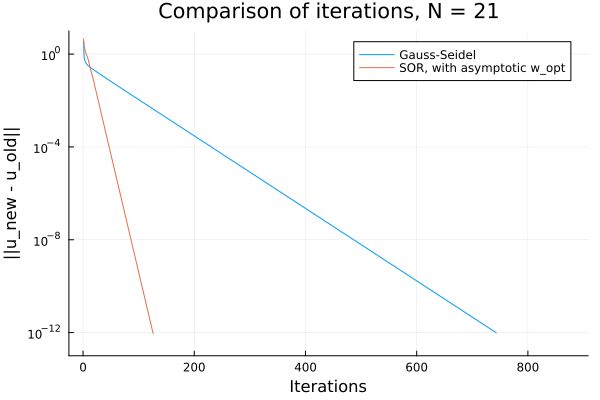
\includegraphics[width=0.4\textwidth]{fig51.png}\label{fig:fig51}}\hfill
    \subfloat[]{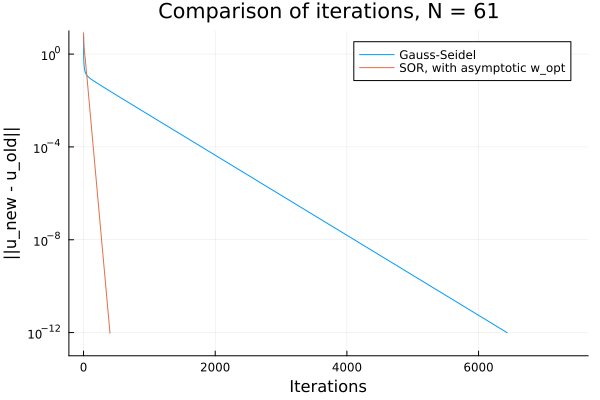
\includegraphics[width=0.4\textwidth]{fig52.png}\label{fig:fig52}}

    \subfloat[]{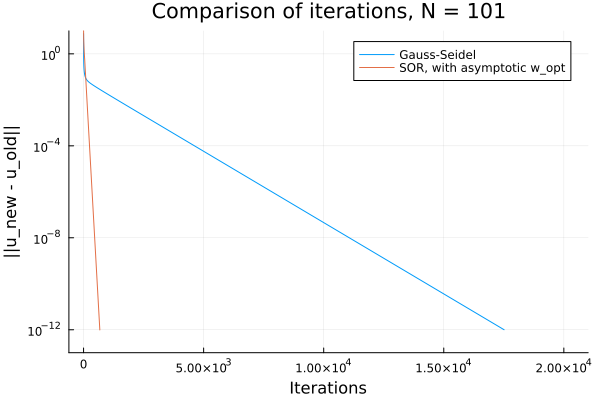
\includegraphics[width=0.4\textwidth]{fig53.png}\label{fig:fig53}}\hfill
    \subfloat[]{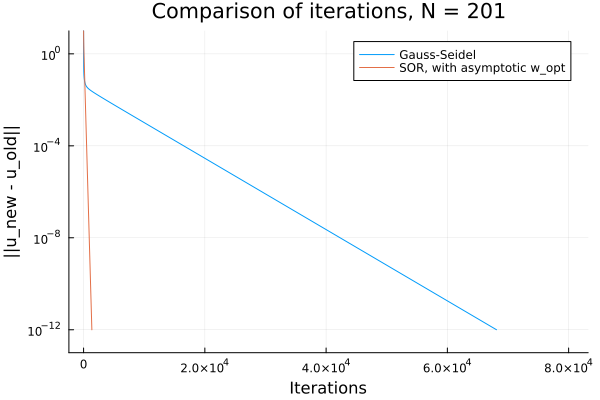
\includegraphics[width=0.4\textwidth]{fig54.png}\label{fig:fig54}}
    \caption{Pseudo-residual plotted against iterations taken, for both Gauss-Seidel and SOR with our asymptotic formula for $w_{opt}$.}
    \label{fig:fig5}
\end{figure}

The table below details the iteration counts for both Gauss-Seidel and SOR with the asymptotic optimal parameter for $w$. We note that SOR bring a very big improvement to the number of iterations required, especially for large $N$. The mathematical theory says that Gauss-Seidel requires $O(N^2)$ iterations, whilst SOR requires $O(N)$ only with the optimal parameter, and one can test this by seeing that $\frac{GS}{SOR \times N}$ is a fixed constant, which is $\approx 0.26$ from the table below.

\begin{table}[H]
    \centering
    \begin{tabular}{|m{2.159cm}|m{2.159cm}|m{2.159cm}|m{2.159cm}|}
    \hline
    $N$ & Gauss-Seidel & SOR & $\frac{GS}{SOR \times N}$ \\ \hline
    21  & 743          & 126 & 0.2808 \\ \hline
    61  & 6433         & 402 & 0.2623 \\ \hline
    101 & 17512        & 677 & 0.2561 \\ \hline
    201 & 68101        & 1365 & 0.2482 \\ \hline
    \end{tabular}
    \end{table}

\subsection{Asserting grid-independence}
To determine grid independence, we calculate a solution for grid sizes $N_k = 2^{k+1}+1$ \ie halving the grid spacing each time. All these grids share the same initial 25 grid points in $N_1$. Thus, we can compare the 2-norm of the difference between the computed solution to $u_{N_k}$ and $u_{N_{k+1}}$ on the shared grid points. To assert grid-independence, we want this norm to be small. The analysis becomes easier if we plot in terms of the corresponding grid spacing $h_k = \frac{2}{N_k - 1}$.

\begin{figure}[H]
    \centering
    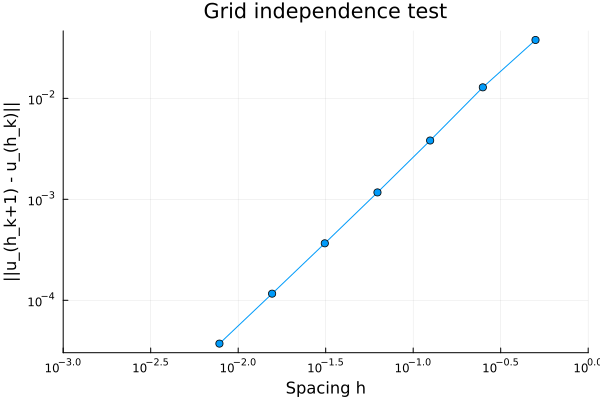
\includegraphics[width=0.49\textwidth]{fig6.png}
    \caption{Log-Log plot of $\|u_{h_{k+1}} - u_{h_k}\|$ plotted against the grid spacing $h_k$.}
    \label{fig:fig6}
\end{figure}
% To see whether this is what we should expect, we analyse the truncation error in our discretisation informally. Given a $N \times N$ evenly spaced grid and the true solution $u$ (where $u^{i,j}$ denotes evaluating the true solution at grid point $(i,j)$), define the local trunctation error at the point $(i,j)$ as follows
% \begin{equation}
%     R_{i,j} = \frac {1}{h^2} \left(
%     u^{i+1, j} + 
%     u^{i-1, j} + 
%     u^{i, j+1} + 
%     u^{i, j-1} - 
%     4u^{i, j}
%     \right) + 4
% \end{equation}
% Recall that the Taylor series expansion of $u_{xx}$:
% \begin{equation}
%     \frac{u^{i+1, j} + 
%     u^{i-1, j} - 2u^{i,j}}{h^2} = \ppn{2}{u^{i,j}}{x} + \frac{h^2}{12}\ppn{4}{u^{i,j}}{x} + O(h^4)
% \end{equation}
% Substituting this back yields that the truncation error is of order $O(h^2)$.
% \begin{equation}
%     R_{i,j} = \frac{h^2}{12} \left(u^{i,j}_{xxxx} + u^{i,j}_{yyyy}\right) + O(h^4)
% \end{equation}
% Suppose $U$ is our solution to the discretised equation $AU=b$. If we then define the error as $z_{i,j} = u_{i,j} - U_{i,j} $, this satisfies the system

% \begin{equation}
%     Az = R = O(h^2)
% \end{equation}

% Which shows that the global error is of order $O(h^2)$, under the assumption that $\|A^{-1}\|$ is bounded as $h \to 0$ (Difficult to show, but is true for simpler domains such as a square). In the above calculation, we didn't take into consideration some of the boundary conditions, but this shouldn't make a huge difference.

From the plotted line we can see that the measured norm difference can be modelled as $Kr^k$ where $K \approx 0.121$ and $r \approx 0.315$. Under the assumption that $u_{h_k}$ converge to the true solution as $k \to \infty$ and that for any $k$, $\|u_{h_{k+1}} - u_{h_k}\| = Kr^k$, we can apply the triangle inequality and geometric series to see that

\begin{equation}
    \|u_{h_k} - u\| \leq \sum_{j=k}^{\infty} \|u_{h_{j+1}} - u_{h_{k}}\| = \sum_{j=k}^{\infty} Kr^j = \frac{Kr^k}{1-r}
\end{equation}

Thus, in order for our solution to satisfy $\|u_{h} - u\| < t$ at the 25 sampled grid points, we need $h$ to be smaller than

\begin{equation}
    h<10^{\frac{\log\left(0.5\right)\log\left(\frac{t\left(1-r\right)}{K}\right)}{\log\left(r\right)}}
\end{equation}

Thus, suppose we wished to have a solution accurate within 1\% of the true solution (at the 25 grid points). We calculate that $h < 0.01887$, so we need at least $106$ grid points. We will choose $201$ grid points to achieve this and have a reasonably grid-independent solution.

\subsection{Contour plots of $u$}

\begin{figure}[H]
    \centering
    \subfloat[]{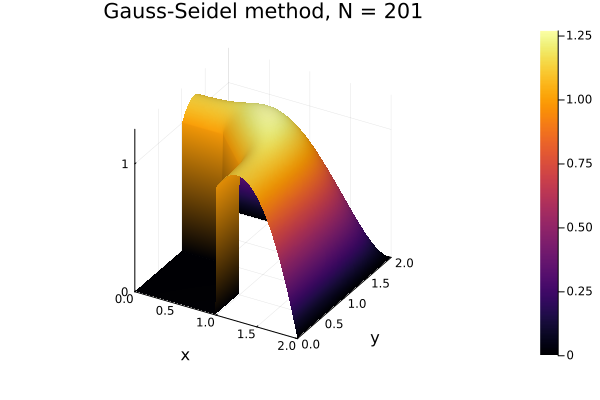
\includegraphics[width=0.49\textwidth]{fig31.png}\label{fig:fig31}}\hfill
    \subfloat[]{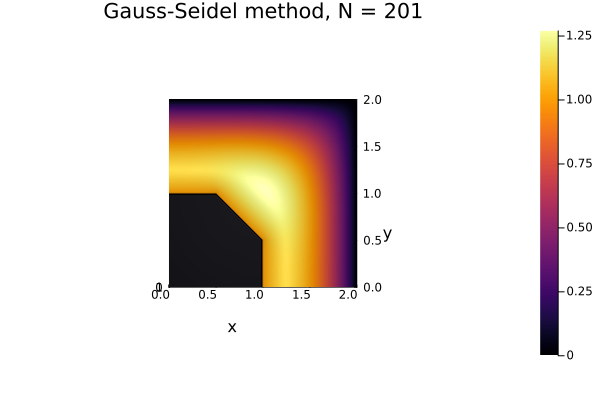
\includegraphics[width=0.49\textwidth]{fig32.png}\label{fig:fig32}}
    \caption{Contoured solution computed with Gauss-Seidel, using $N=201, h=0.005$.}
    \label{fig:fig3}
\end{figure}

\begin{figure}[H]
    \centering
    \subfloat[]{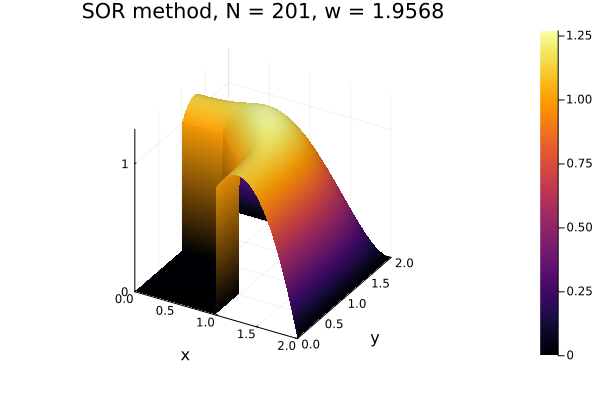
\includegraphics[width=0.49\textwidth]{fig41.png}\label{fig:fig41}}\hfill
    \subfloat[]{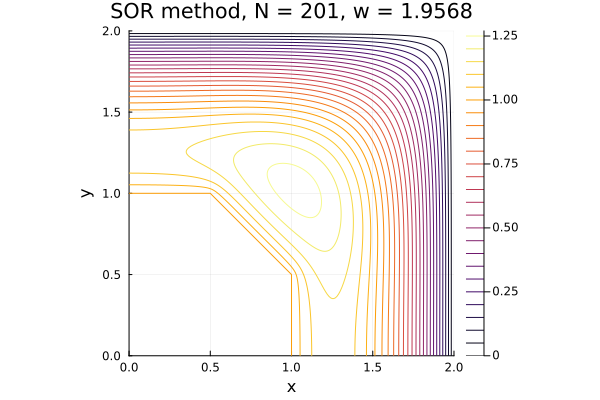
\includegraphics[width=0.49\textwidth]{fig42.png}\label{fig:fig42}}
    \caption{Contoured solution computed with SOR, $w=1.9568$ using $N=201, h=0.005$.}
    \label{fig:fig4}
\end{figure}

\subsection{Material Stresses}
We can plot the individual components of $u_x$ and $u_y$ by using a backward 1st order difference (where $i$ and $j$ increase in the direction of positive $x$ and positive $y$ respectively).
\begin{equation}
    u_x \approx \frac{U_{i,j} - U_{i-1,j}}{h} \hspace{1cm} u_y \approx \frac{U_{i,j} - U_{i,j-1}}{h}
\end{equation}

The individual components are plotted below in Figure \ref{fig:fig7}. We notice the small spikes near the two $135^{\circ} $ corners, and the large components near the edge.

\begin{figure}[H]
    \centering
    \subfloat[$u_x$]{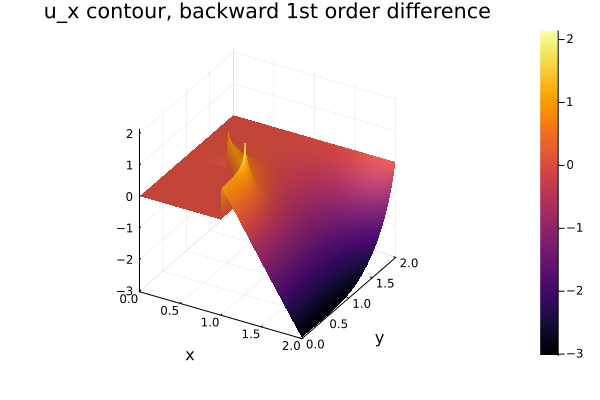
\includegraphics[width=0.49\textwidth]{fig71x.png}\label{fig:fig71x}}\hfill
    \subfloat[$u_x$]{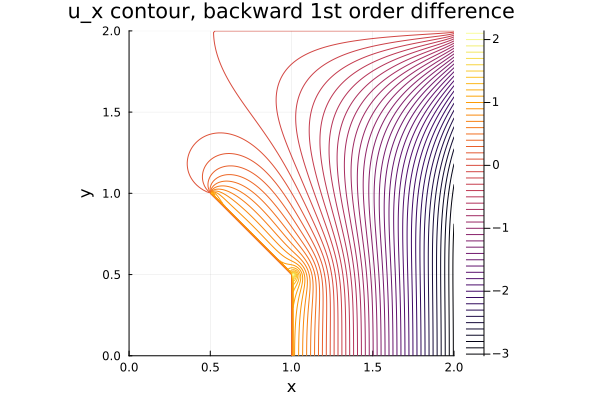
\includegraphics[width=0.49\textwidth]{fig72x.png}\label{fig:fig72x}}

    \subfloat[$u_y$]{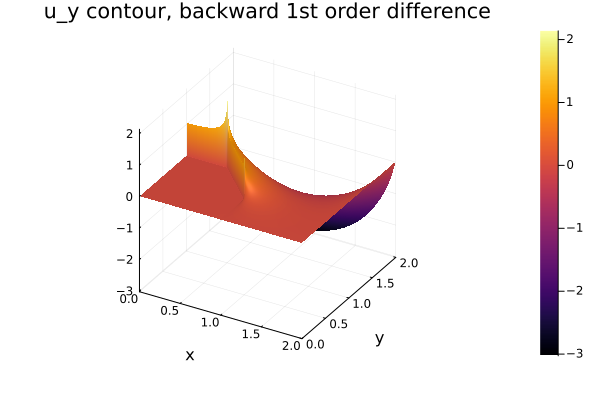
\includegraphics[width=0.49\textwidth]{fig71y.png}\label{fig:fig71y}}\hfill
    \subfloat[$u_y$]{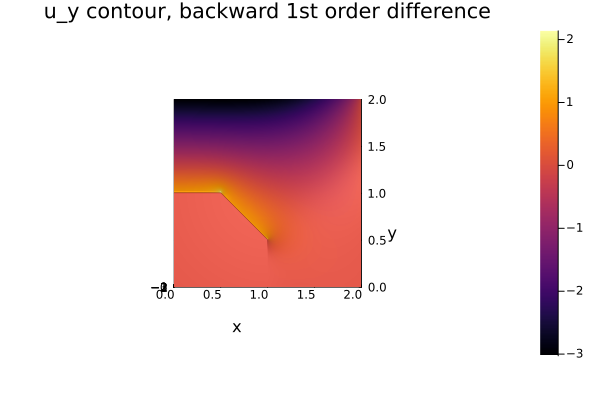
\includegraphics[width=0.49\textwidth]{fig72y.png}\label{fig:fig72y}}
    \caption{Horizontal and vertical components of stress vectors.}
    \label{fig:fig7}
\end{figure}
For this grid, the maximum and minimum values are summarised in the table below. Since the problem is symmetric, we expect that the maximum and minimum values for $u_x$ and $u_y$ are the same.

\begin{table}[H]
    \centering
    \begin{tabular}{|l|l|l|l|}
    \hline
    $\max(u_x)$        & $\min(u_x)$         & $\max(u_y)$        & $\min(u_x)$         \\ \hline
    2.1386238454222495 & -3.0268664561932646 & 2.1386238454222495 & -3.0268664561932646 \\ \hline
    \end{tabular}
    \end{table}
We can also plot as a heatmap the magnitude and direction of the stress vectors, as seen in Figure \ref{fig:fig8}. From this we see that the areas of greatest stress are the two long edges, particularly near the corners $(0,2)$ and $(2,0)$. In addition, the two corners located at $(0.5,1)$ and $(1,0.5)$ experience stress as well in a very concentrated region.

\begin{figure}[H]
    \centering
    \subfloat[Vector field]{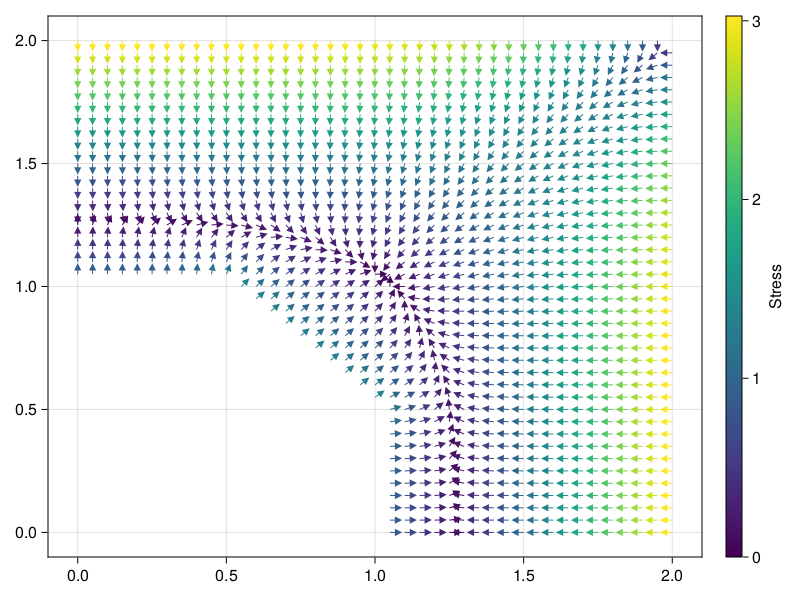
\includegraphics[width=0.33\textwidth]{fig81.png}\label{fig:fig81}}
    \subfloat[Contour map of vector magnitudes]{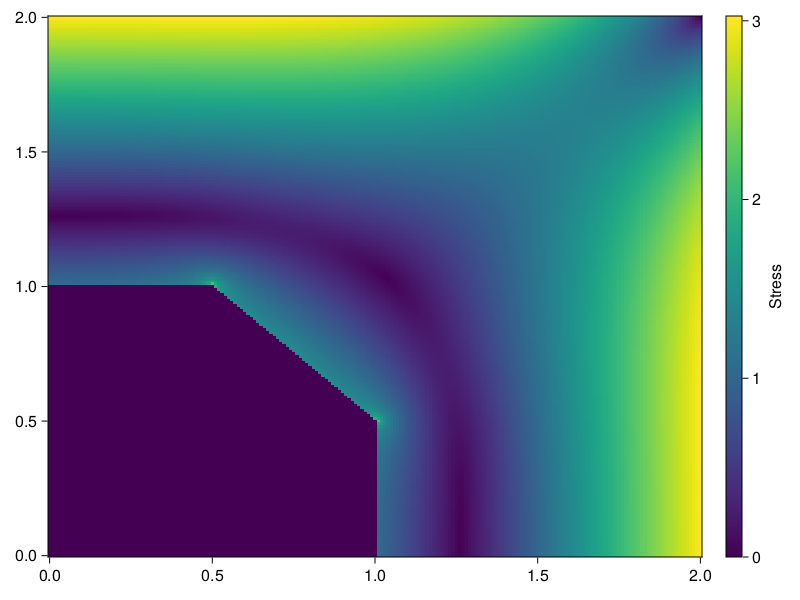
\includegraphics[width=0.33\textwidth]{fig82.png}\label{fig:fig82}}
    \subfloat[Heatmap of vector magnitudes]{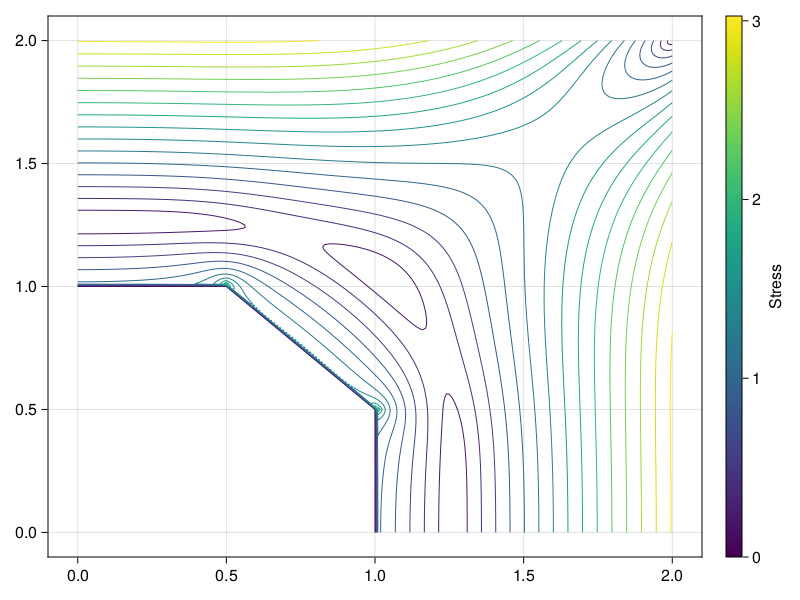
\includegraphics[width=0.33\textwidth]{fig83.png}\label{fig:fig83}}\hfill
    \caption{Material stress calculated using backward 1st order finite differences.}
    \label{fig:fig8}
\end{figure}


\subsection{Material stress in different grid sizes}
In order to investigate grid-independence for material stress, we repeat these calculations for different $N$ and calculate the corresponding maximum and minimum $u_x$ and $u_y$. In the table below, we see that the minimum values of $\sigma_x$ and $\sigma_y$ are invariant under different grid sizes. However, the maximum is not: it is increasing as the grid becomes finer, without converging.

Intuitively, this makes sense since the negative values of $\sigma_x$ and $\sigma_y$ are achieved near the top-left and bottom-right corners and are generally spread out over a large area. In Figure \ref{fig:fig7}, these two regions appear to behave nicely \ie they do not change rapidly.

However, the positive values are concentrated in a small region, and when contoured in Figure \ref{fig:fig7} and Figure \ref{fig:fig8}, the values of $\sigma_x$ and $\sigma_y$ have a sudden spike in the corners and appear to blow up. This requires a finer grid in the neighbourhood the points to resolve the material stresses accurately, which could explain why these values are heavily dependent on the grid.%Even in Figure \ref{fig:fig3}, the contoured solution of $u$ has non-smooth behaviour at the points $(0.5,1)$ and $(1,0.5)$.


\begin{table}[H]
    \centering
    \begin{tabular}{|l|l|l|l|l|}
    \hline
    $N$ & $\max(u_x)$        & $\min(u_x)$         & $\max(u_y)$        & $\min(u_x)$         \\ \hline
    101 & 1.8334958585643601 & -3.0067386661442326 & 1.8334958585643601 & -3.0067386661442326 \\ \hline
    201 & 2.1386238454222495 & -3.0268664561932646 & 2.1386238454222495 & -3.0268664561932646 \\ \hline
    301 & 2.33045628089954   & -3.033566569231908  & 2.33045628089954   & -3.033566569231908  \\ \hline
    401 & 2.474243586283187  & -3.0369122087117493 & 2.474243586283187  & -3.0369122087117493 \\ \hline
    501 & 2.590726251260278  & -3.0389180506760622 & 2.590726251260278  & -3.0389180506760622 \\ \hline
    801 & 2.851829158146124 & -3.041925611353496 & 2.851829158146124 & -3.041925611353496 \\ \hline
    \end{tabular}
    \end{table}



% \begin{figure}[H]
%     \centering
%     \begin{tikzpicture}[scale=1.5]

        
        

%         \draw (2,0) -- (2,1);
%         \draw (2,1) -- (1,2);
%         \draw (1,2) -- (0,2);
%         \draw (0,2) -- (0,4);
%         \draw (0,4) -- (4,4);
%         \draw (4,4) -- (4,0);
%         \draw (4,0) -- (2,0);

%         \draw[red] (1.5,1.5) -- (4,4);

        
%         \node at (1.25-0.1475,1.75-0.1475) {$1$};
%         \node at (0.5,2-0.2475) {$1$};
%         \node at (2,4+0.2475) {$0$};

%     \end{tikzpicture}
%     \caption{Order for Gauss-Seidel sweeps, single grid.}
%     \label{fig:grid3}
% \end{figure}


\section{Part C}
\subsection{Grid transform diagram}

\begin{minipage}{0.5\textwidth}

    \begin{figure}[H]
        \centering
        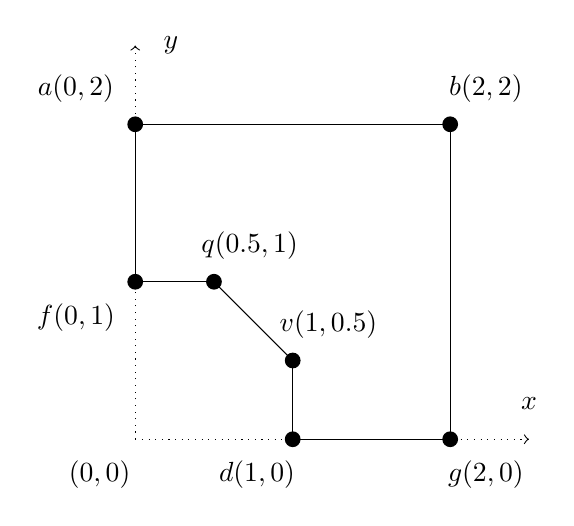
\begin{tikzpicture}
            % First square
            \draw (2,0) -- (4,0);
            \draw (4,0) -- (4,4);
            \draw (4,4) -- (0,4);
            \draw (0,4) -- (0,2);
            \draw (0,2) -- (1,2);
            \draw (1,2) -- (2,1);
            \draw (2,1) -- (2,0);
            \draw[dotted, ->] (0,0) -- (5,0);
            \draw[dotted, ->] (0,0) -- (0,5);

            % \draw[dotted] (0,0) -- (0,-0.4);
            % \draw[dotted] (2,0) -- (2,-0.4);
            % \draw[dotted] (4,0) -- (4,-0.4);

            \node at (5,0+0.4533) {$x$};
            \node at (0+0.4533,5) {$y$};

            \node at (4+0.4533,0-0.4533) {$g (2,0)$};
            \node at (4+0.4533,4+0.4533) {$b (2,2)$};
            \node at (0-0.7533,4+0.4533) {$a (0,2)$};
            \node at (0-0.7533,2-0.4533) {$f (0,1)$};
            \node at (1+0.4533,2+0.4533) {$q (0.5,1)$};
            \node at (2+0.4533,1+0.4533) {$v (1,0.5)$};
            \node at (2-0.4533,0-0.4533) {$d (1,0)$};
            \node at (0-0.4533,0-0.4533) {$(0,0)$};

            \fill (2,0) circle (0.1);
            \fill (4,0) circle (0.1);
            \fill (4,4) circle (0.1);
            \fill (0,4) circle (0.1);
            \fill (0,2) circle (0.1);
            \fill (1,2) circle (0.1);
            \fill (2,1) circle (0.1);

        \end{tikzpicture}
        \caption*{Physical plane}
        \label{fig:phys}
    \end{figure}
    \end{minipage}%
    \begin{minipage}{0.5\textwidth}
        \begin{figure}[H]
            \centering
            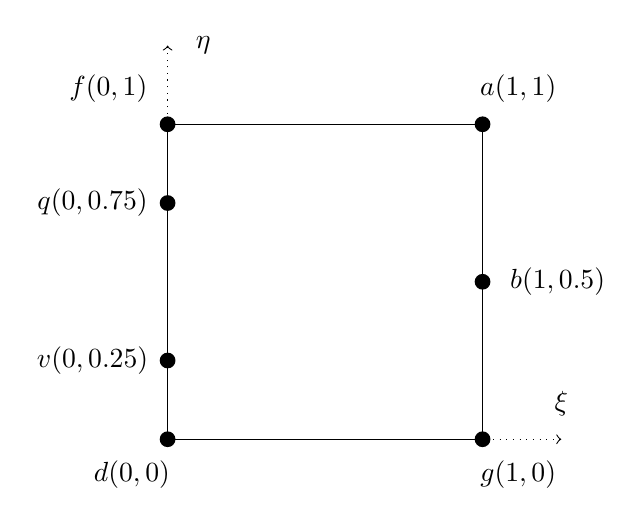
\begin{tikzpicture}
                % Second square
                \draw (0,0) rectangle (4,4);

                \fill (4,4) circle (0.1);
                \fill (4,2) circle (0.1);
                \fill (4,0) circle (0.1);
                \fill (0,0) circle (0.1);
                \fill (0,1) circle (0.1);
                \fill (0,3) circle (0.1);
                \fill (0,4) circle (0.1);

                \node at (4+0.4533,0-0.4533) {$g (1,0)$};
                \node at (4+0.9533,2+0.0000) {$b (1,0.5)$};
                \node at (4+0.4533,4+0.4533) {$a (1,1)$};
                \node at (0-0.7533,4+0.4533) {$f (0,1)$};
                \node at (0-0.9533,3+0.0000) {$q (0,0.75)$};
                \node at (0-0.9533,1+0.0000) {$v (0,0.25)$};
                \node at (0-0.4533,0-0.4533) {$d (0,0)$};

                \draw[dotted, ->] (0,0) -- (5,0);
                \draw[dotted, ->] (0,0) -- (0,5);
                
                \node at (5,0+0.4533) {$\xi$};
                \node at (0+0.4533,5) {$\eta$};
            \end{tikzpicture}
            \label{fig:comp}
            \caption*{Computational plane}
        \end{figure}
    \end{minipage}

The above diagram shows the map from the physical plane to the computational plane. We choose $\xi$ and $\eta$ such that
\begin{itemize}
    \item $\xi$ and $\eta$ are harmonic \ie 
    \begin{equation}
        \xi_{xx} + \xi_{yy} = 0 \hspace{1cm} \eta_{xx} + \eta_{yy} = 0
    \end{equation}
    \item $\xi = 0$ on $f - q - v - d$ and $\xi=1$ on $g - b - a$. Similarly $\eta=0$ on $g - d$ and $\eta=1$ on $a - f$. All other boundary values in the physical plane are interpolated linearly \eg $\xi$ goes from $0$ to $1$ along the edge $a - f$ linearly.
\end{itemize}

In Figure \ref{fig:fig10} we plot the computational grid and show how it maps to the real physical grid we have.

\begin{figure}[H]
    \centering
    \subfloat[]{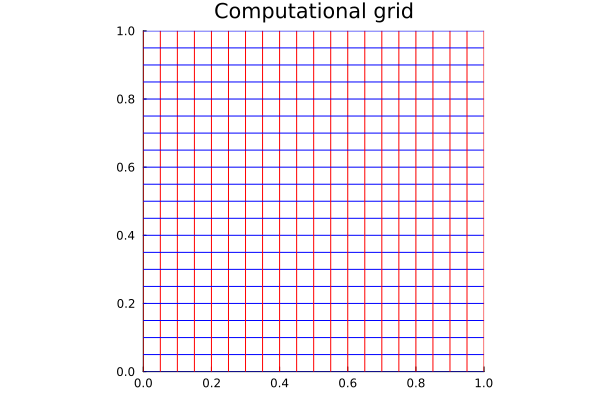
\includegraphics[width=0.499\textwidth]{fig10comp.png}\label{fig:fig10comp}}\hfill
    \subfloat[]{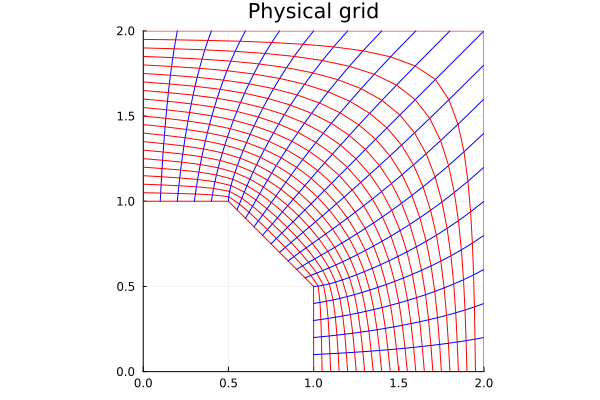
\includegraphics[width=0.499\textwidth]{fig10phys.png}\label{fig:fig10phys}}
    \caption{Computational grid to Physical grid mapping}
    \label{fig:fig10}
\end{figure}
The above plot was generated by solving the system of quasilinear elliptic PDEs
\begin{align}
    \label{eq:xypde}
    &\alpha x_{\xi\xi} - 2\beta x_{\xi\eta} + \gamma x_{\eta\eta} = 0 \\
    &\alpha y_{\xi\xi} - 2\beta y_{\xi\eta} + \gamma y_{\eta\eta} = 0 \nonumber\\
    &\text{where} \nonumber\\
    &\alpha = x_{\eta}^2 + y_{\eta}^2 \nonumber\\
    &\beta = x_{\xi} x_{\eta} + y_{\xi} y_{\eta} \nonumber\\
    &\gamma = x_{\xi}^2 + y_{\xi}^2 \nonumber
\end{align}
The boundary conditions are just Dirichlet boundary conditions, which correspond to the $x$ or $y$ values we should expect along the edges of the computational plane. The above equations were solved using $O(h^2)$ order finite differences for all terms, with $i$ pointing in the positive $\xi$ direction and $j$ in the positive $\eta$ direction.
\begin{align}
    \pp{x_{i,j}}{\xi} &\approx \frac{x_{i+1,j} - x_{i-1,j}}{2h} \\
    \ppn{2}{x_{i,j}}{\xi} &\approx \frac{x_{i+1,j} - 2x_{i,j} + x_{i-1,j}}{h^2} \\
    \frac{\partial^2 x_{i,j}}{\partial \xi \partial \eta} &\approx \frac{x_{i+1,j+1} + x_{i-1,j-1} - x_{i-1,j+1} - x_{i+1,j-1}}{4h^2}
\end{align}
Using these finite differences, Gauss-Seidel iteration was applied (with the possibility for acceleration), solving for $x_{i,j}$ and $y_{i,j}$ each time (despite it not being a linear problem). A function for solving this is written at \path{gauss_seidel_xy_C}. % \textbf{TODO: maybe add in proof of convergence with careful error control and showing that the errors don't grow.}


\subsection{Computing the solution using the elliptic transform}
The transformed PDE in terms of $\xi,\eta$ is calculated by using the chain rule \eg $u_x = u_\xi \xi_x + u_\eta \eta_x$ and the symmetry of second-order partial derivatives.
\begin{equation}
    u_{\xi\xi}(\xi_x^2 + \xi_y^2) + 2u_{\xi\eta}(\eta_x \xi_x + \eta_y \xi_y) + u_{\eta\eta} (\eta_x^2 + \eta_y^2) + 4 = 0
\end{equation}
We can then use the inverse of the Jacobian matrix to rewrite the PDE using the derivatives of $x$ and $y$, where the Jacobian determinant is given as $J = x_{\xi}y_{\eta} - x_{\eta}y_{\xi}$.
\begin{equation}
\begin{pmatrix}
    \xi_{x} & \xi_{y}\\
    \eta_{x} & \eta_{y}
    \end{pmatrix} =
    \begin{pmatrix}
    x_{\xi} & x_{\eta}\\ 
    y_{\xi} & y_{\eta}
    \end{pmatrix}^{-1} =
    \frac {1}{J}
    \begin{pmatrix}
    y_{\eta} & -x_{\eta}\\ 
    -y_{\xi} & x_{\xi}
    \end{pmatrix}
\end{equation}
resulting in the PDE
\begin{equation}
    u_{\xi\xi}(y_{\eta}^2 + x_{\eta}^2) - 2u_{\xi\eta}(y_\xi y_\eta + x_\xi x_\eta) + u_{\eta\eta} (y_{\xi}^2 + x_{\xi}^2) + 4J^2 = 0
\end{equation}
The boundary conditions are given by
\begin{itemize}
    \item $u(0,\eta) = 1$
    \item $u(1,\eta) = 0$
    \item $u_{\xi} y_{\eta} - u_{\eta} y_{\xi} = 0$ when $\eta=1$
    \item $u_{\eta} x_{\xi} - u_{\xi} x_{\eta} = 0$ when $\eta=0$
\end{itemize}
The last two conditions follow from the chain rule when applied to $u_x = 0$ and $u_y=0$ respectively. We discretise all the derivatives as $O(h^2)$ accurate (the same used in finding $x$ and $y$). At the top and bottom boundary, we have to use $O(h^2)$ accurate forward and backward differences for the derivatives $x_{\eta}$ and $y_{\eta}$, namely
\begin{align}
    \label{eq:forwardoh2}
    f'(x) &= \frac{-3f(x) + 4f(x+h) - f(x+2h)}{2h} + O(h^2) \\
    f'(x) &= \frac{3f(x) - 4f(x-h) + f(x-2h)}{2h} + O(h^2) \nonumber
\end{align}
Once we have approximated all the derivatives of $x$ and $y$, we can use Gauss-Seidel iteration (Function written at \path{gauss_seidel_method_C}) applied to the linear PDE
%These are used to approximate $x_{\eta}$ and $y_{\eta}$. 
An alternative approach would be to calculate the values of $x$ and $y$ at "ghost" points just above and below the lines $\eta=1$ and $\eta=0$ and use central differences. These values have to be calculated using iteration, since the system to be solved is also non-linear.

We first calculate a solution using $N=61$ and show it in Figure \ref{fig:fig11}.
\begin{figure}[H]
    \centering
    \subfloat[]{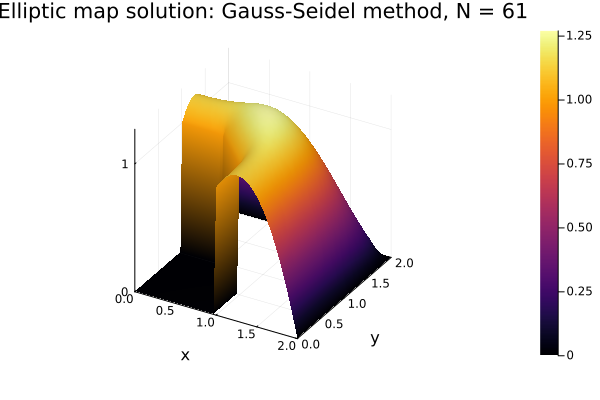
\includegraphics[width=0.49\textwidth]{fig111.png}\label{fig:fig111}}
    \subfloat[]{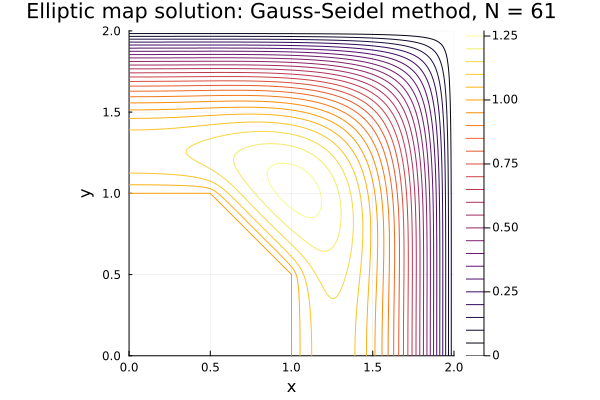
\includegraphics[width=0.49\textwidth]{fig113.png}\label{fig:fig113}}\hfill
    \caption{Solution $u$ calculated using Elliptic maps to a square grid.}
    \label{fig:fig11}
\end{figure}

\subsection{Clustering of grid points}
We demonstrate how the physical grid tends to cluster points around the two $135^{\circ} $ corners in Figure \ref{fig:fig12}. 

\begin{figure}[H]
    \centering
    \subfloat[$N=21$]{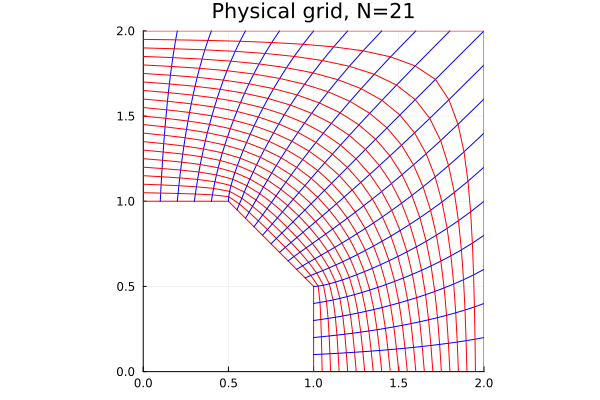
\includegraphics[width=0.49\textwidth]{fig1211.png}\label{fig:fig1211}}
    \subfloat[Close up]{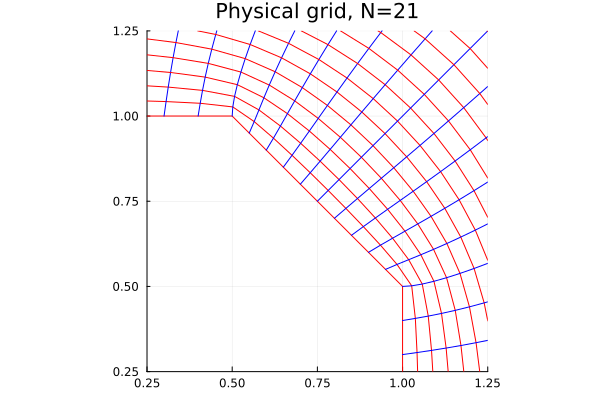
\includegraphics[width=0.49\textwidth]{fig1212.png}\label{fig:fig1212}}\hfill
    \subfloat[$N=61$]{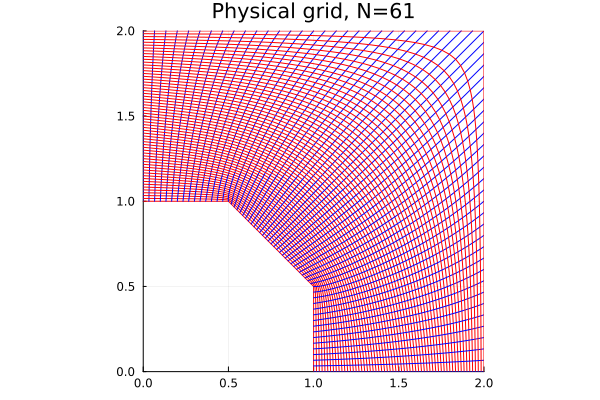
\includegraphics[width=0.49\textwidth]{fig1221.png}\label{fig:fig1221}}
    \subfloat[Close up]{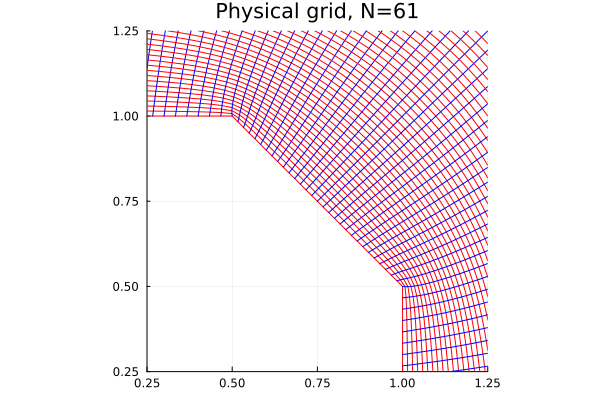
\includegraphics[width=0.49\textwidth]{fig1222.png}\label{fig:fig1222}}\hfill
    \caption{Physical grid for $N=21$ and $N=61$, focused on the two inner corners.}
    \label{fig:fig12}
\end{figure}

Even if we change the boundary conditions in solving PDE \eqref{eq:xypde} (to lower the number of points along the $q-v$ edge from $N/2$ to only $N/5$, for example), the points still cluster near $q$ and $v$, with some warping of the squares near the edge.

\begin{figure}[H]
    \centering
    \subfloat[$N=21$]{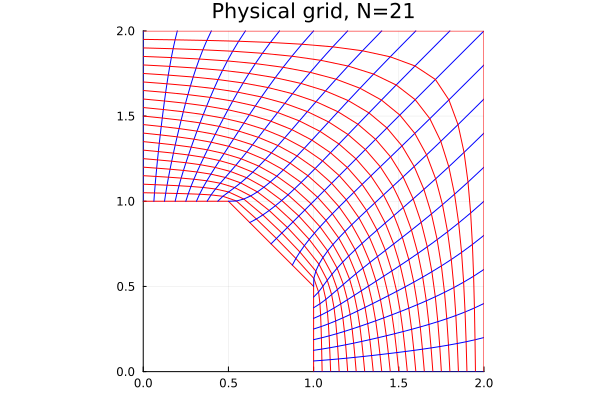
\includegraphics[width=0.49\textwidth]{fig1311.png}\label{fig:fig1311}}
    \subfloat[Close up]{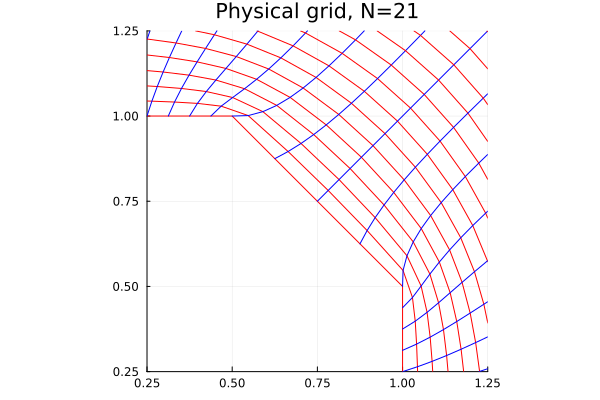
\includegraphics[width=0.49\textwidth]{fig1312.png}\label{fig:fig1312}}\hfill
    \subfloat[$N=61$]{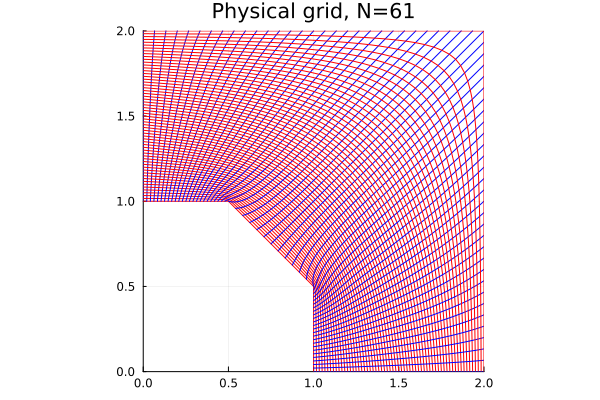
\includegraphics[width=0.49\textwidth]{fig1321.png}\label{fig:fig1321}}
    \subfloat[Close up]{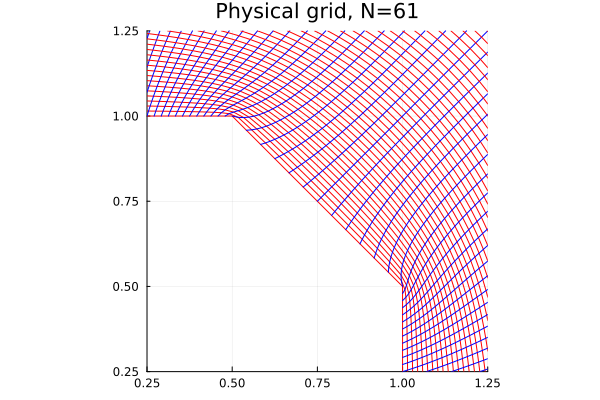
\includegraphics[width=0.49\textwidth]{fig1322.png}\label{fig:fig1322}}\hfill
    \caption{Physical grid for $N=21$ and $N=61$, focused on the two inner corners, with less points on the $q-v$ edge.}
    \label{fig:fig13}
\end{figure}



\subsection{Asserting grid-independence: Elliptic mapping}
Below (Figure \ref{fig:fig14}) are plots of the pseudo residual on the computational grid as the number of points $N$ is increased. A coarse $5 \times 5$ grid was refined by halving the spacing $h$ each time, and the norm of $u_{new} - u_{old}$ was measured on the shared $25$ grid points, though this time we cannot calculate with as high values of $N$ due to the expensive computation of computing $x$ and $y$ from the quasilinear PDE (See Equation \eqref{eq:xypde}). Although the accuracy is not as good as in Figure \ref{fig:fig6} for each individual spacing $h$, we see that the residual is decreasing by a fixed factor (roughly $r=0.25$) for each halving of the grid spacing much like before. A similar calculation to before tells us that around $N=220$ is needed to be within 1\% of the true solution. Due to computational constraints, we will use $N=101$ grid points from now on.

\begin{figure}[H]
    \centering
    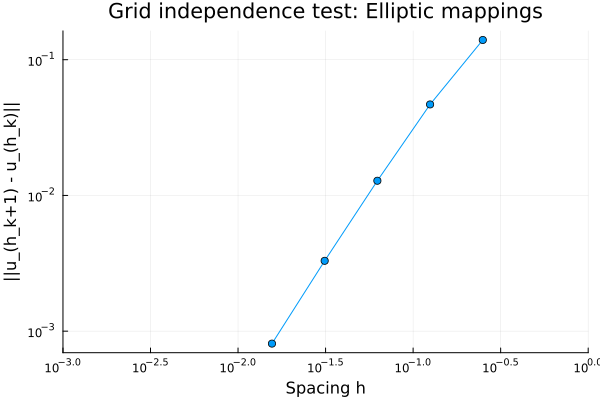
\includegraphics[width=0.49\textwidth]{fig14.png}
    \caption{Log-Log plot of $\|u_{h_{k+1}} - u_{h_k}\|$ plotted against the grid spacing $h_k$, for the elliptic mapping solution.}
    \label{fig:fig14}
\end{figure}

\subsection{Comparison with Part B solution: Stress along $f-q-v-d$}
Comparison of the solutions is hard to do within the interior of the domain, since the grid points are not shared and interpolation errors would dominate. However, we can measure the stress along the edge since these points are shared to compare.

In order to compare $u_x$ and $u_y$, we need to use the chain rule for the solution using elliptic mappings, which results in
\begin{equation}
    u_x = \frac{u_{\xi} y_{\eta} - u_{\eta} y_{\xi}}{J} \hspace{1cm} 
    u_y = \frac{u_{\eta} x_{\xi} - u_{\xi} x_{\eta}}{J}
\end{equation}

We use $O(h^2)$ accurate forward differences (See Equation \eqref{eq:forwardoh2}) to approximate all the derivatives. Figure \ref{fig:fig15} shows both the individual stress components $\sigma_x$ and $\sigma_y$ along with the magnitude of the stress vector. We see that the solutions agree away from the two points $q$ and $v$ (Within $O(h^2)$ error), but closer to the two corners the solutions vary more. This is what we expect, as previously we determined that the maximum values of $\sigma_x$ and $\sigma_y$ are achieved at these two points and are not grid independent. As such, some variation is to be expected in the stress values near $q$ and $v$.

\begin{figure}[H]
    \centering
    \subfloat[$\sigma = \sqrt{\sigma_x^2 + \sigma_y^2}$]{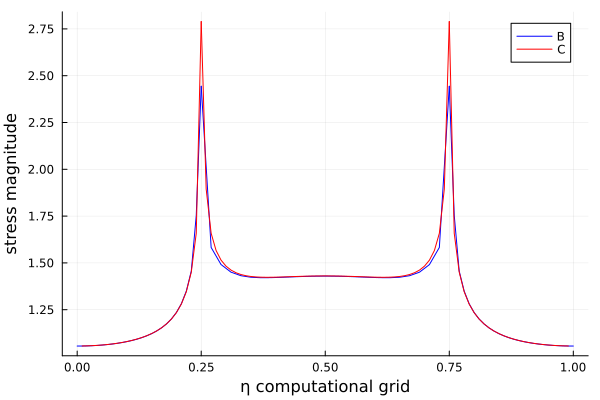
\includegraphics[width=0.49\textwidth]{fig151.png}\label{fig:fig151}}
    \subfloat[Absolute difference of $\sigma$ from part B and C]{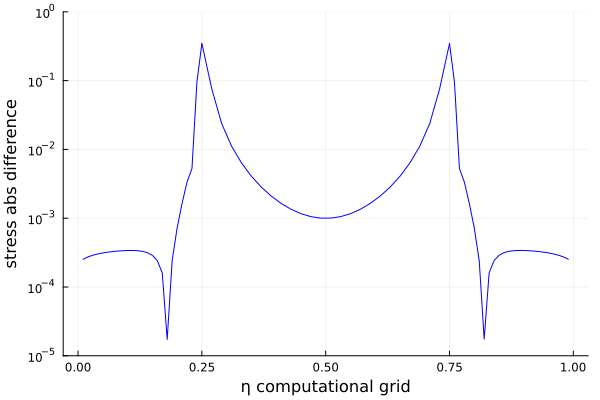
\includegraphics[width=0.49\textwidth]{fig152.png}\label{fig:fig152}}\hfill
    \subfloat[$\sigma_x$]{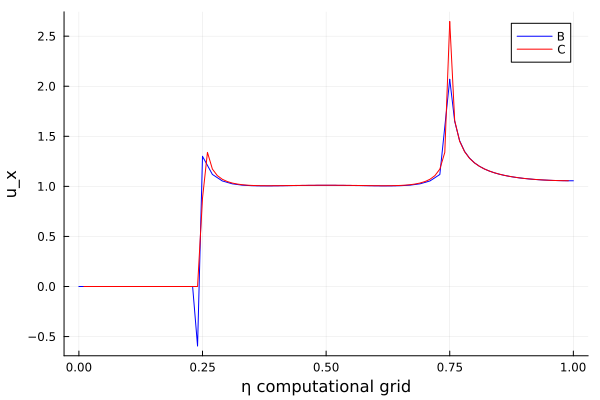
\includegraphics[width=0.49\textwidth]{fig153.png}\label{fig:fig153}}
    \subfloat[$\sigma_y$]{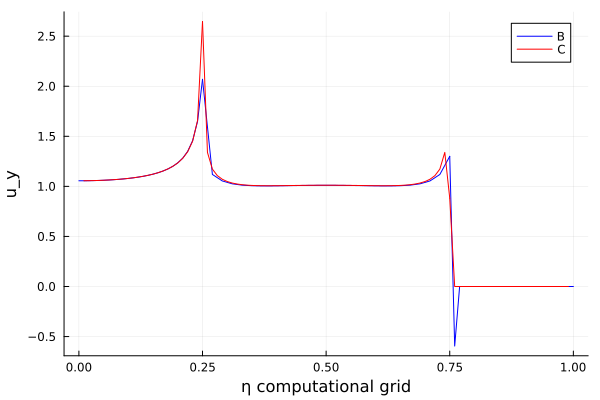
\includegraphics[width=0.49\textwidth]{fig154.png}\label{fig:fig154}}\hfill
    \caption{Comparison of stress along $f-q-v-d$ boundary.}
    \label{fig:fig15}
\end{figure}

\subsection{Contour plots of stress field: Elliptic mapping}
Due to the irregular placement of data, some plots can't be created (because Julia doesn't have a \path{tricontour} function\dots). Nevertheless, we plot the vector field of the stress and the contour plots of the magnitude of the stress as well as the individual $x$ and $y$ components. Much like before, we see that the greatest stress occurs near the top-left and bottom-right corners in a widespread area. Similarly we see spikes in the stress in the two corners at $q$ and $v$.

\begin{figure}[H]
    \centering
    \subfloat[Vector field]{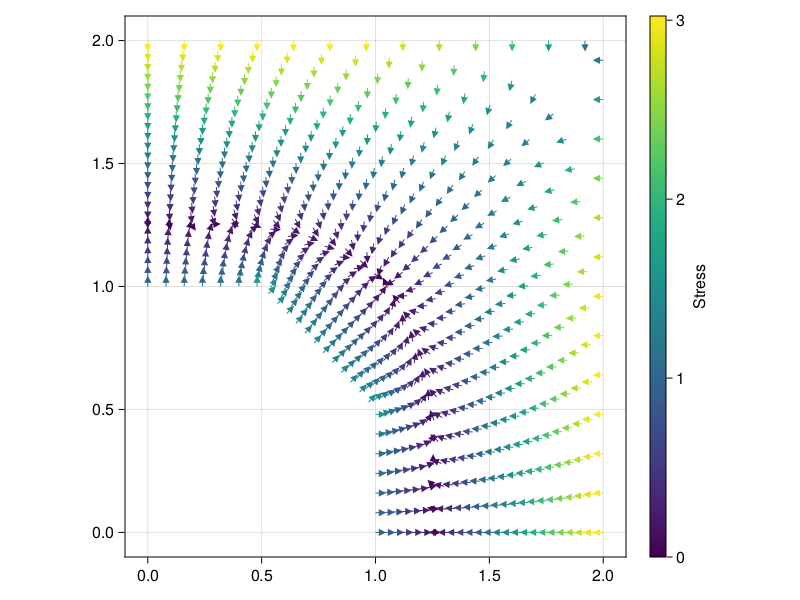
\includegraphics[width=0.49\textwidth]{fig161.png}\label{fig:fig161}}
    \subfloat[$\sigma = \sqrt{\sigma_x^2 + \sigma_y^2}$]{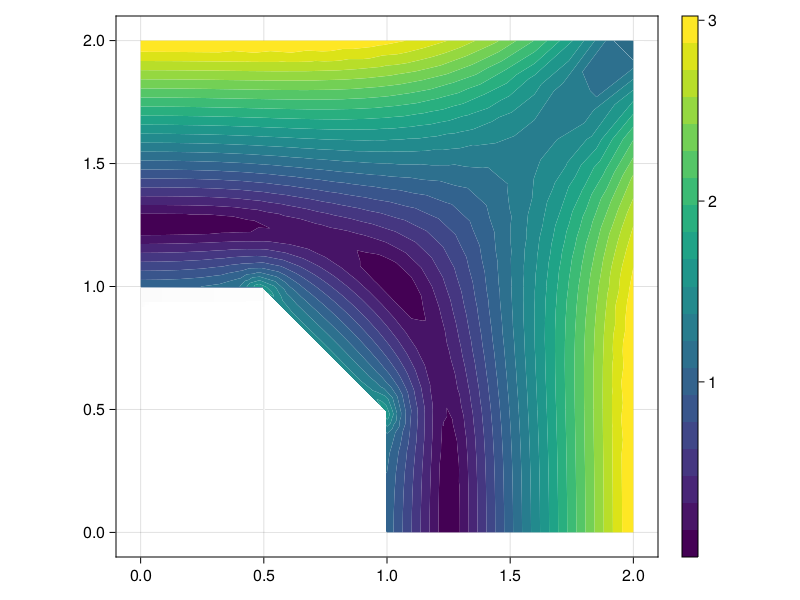
\includegraphics[width=0.49\textwidth]{fig162.png}\label{fig:fig162}}\hfill
    \subfloat[$\sigma_x$]{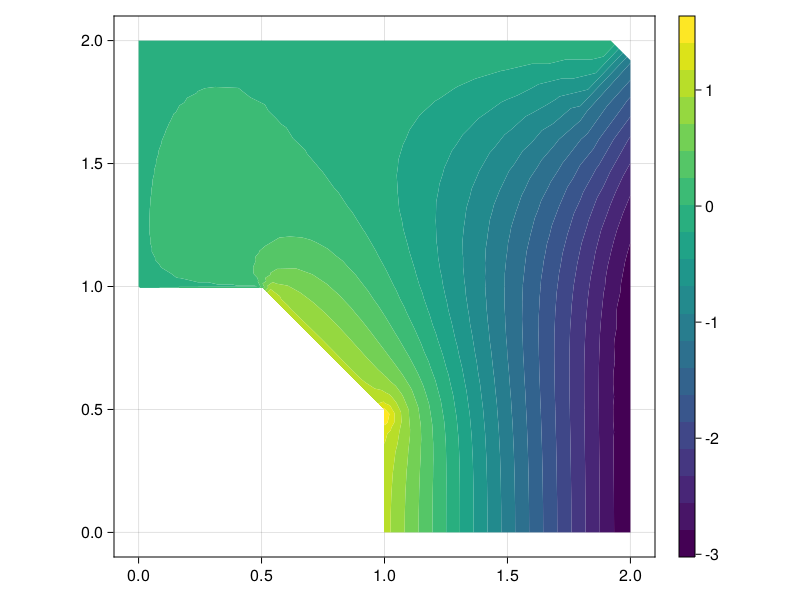
\includegraphics[width=0.49\textwidth]{fig163.png}\label{fig:fig163}}
    \subfloat[$\sigma_y$]{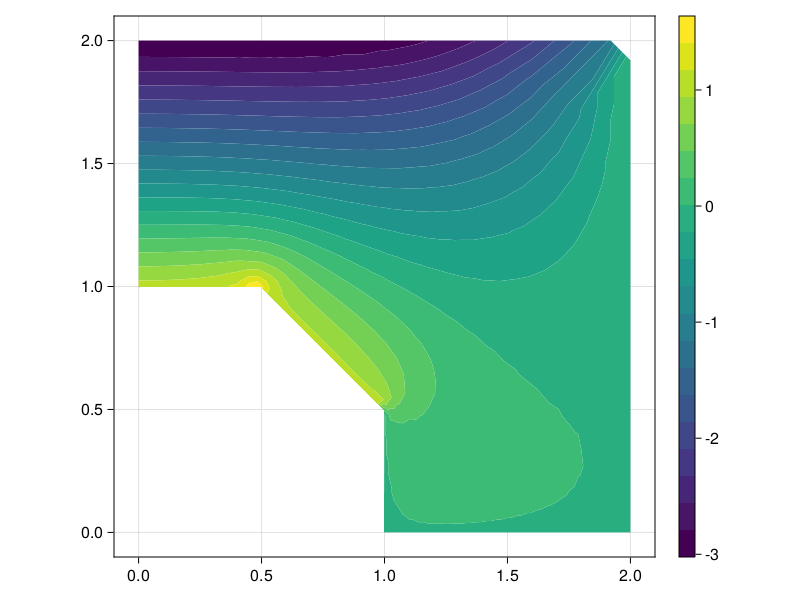
\includegraphics[width=0.49\textwidth]{fig164.png}\label{fig:fig164}}\hfill
    \caption{Plots of stress field $\sigma$}
    \label{fig:fig16}
\end{figure}


\end{document}